\chapter{Platforma od strony użytkowej}
\label{chapter:interfaces}

Stroną startową platformy jest ekran logowania użytkownika.
Uwierzytelnienie odbywa się z użyciem serwisu GitHub (opis techniczny procesu znajduje się w podrozdziale~\ref{authorization}).
Po poprawnym zalogowaniu użytkownik jest przekierowywany do kolejnego widoku zależnego od jego uprawnień.
W przypadku prowadzącego jest to ekran wyboru zarządzania projektami lub podglądu postępów studentów.
Użytkownik będący studentem jest przekierowywany do widoku dostępnych dla niego projektów.

Opis ekranu logowania znajduje się w podrozdziale \ref{fe_login}.
W kolejnej sekcji zostały omówione interfejsy dostępne dla prowadzącego.
Ostatni podrozdział zawiera opis widoku studenta.

\section{Panel logowania}
\label{fe_login}

Panel logowania umożliwia uwierzytelnienie z użyciem serwisu GitHub.
Po kliknięciu przycisku ”Zaloguj” użytkownik jest przekierowywany na stronę logowania GitHub.
W~serwisie można zalogować się poprzez podanie adresu e-mail bądź nazwy użytkownika i hasła.
Należy też wyrazić zgodę na przetwarzanie danych przez platformę.
Po poprawnym zalogowaniu użytkownik zostaje przekierowany z powrotem na stronę platformy.
Po przetworzeniu danych uwierzytelniających przez platformę użytkownikowi wyświetlany jest kolejny ekran, zależny od jego uprawnień.
Na rysunkach od \ref{fig:log_in_button} do \ref{fig:wait_for_login} zostały przedstawione kolejne ekrany związane z procesem logowania.

\vfill

\begin{figure}[h]
    \centering
    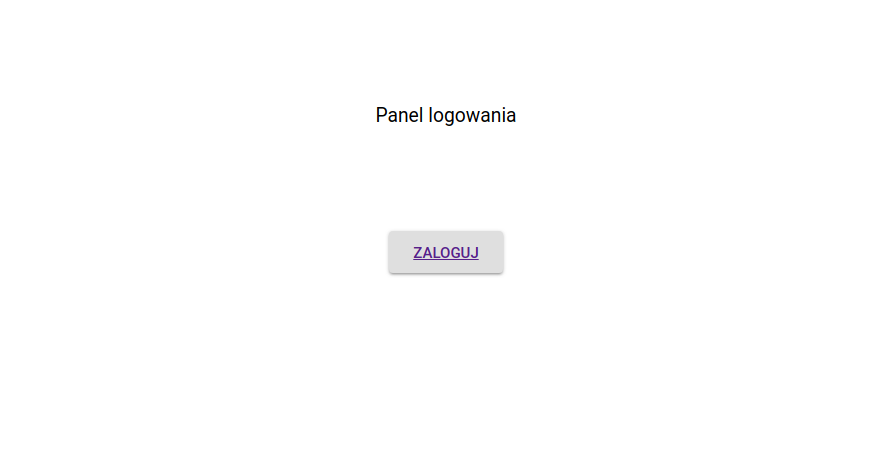
\includegraphics[width = 8cm]{chapter04/log_in_button.png}
    \caption{Ekran logowania w ramach platformy (źródło własne).}
    \label{fig:log_in_button}
\end{figure}

\begin{figure}[h]
    \centering
    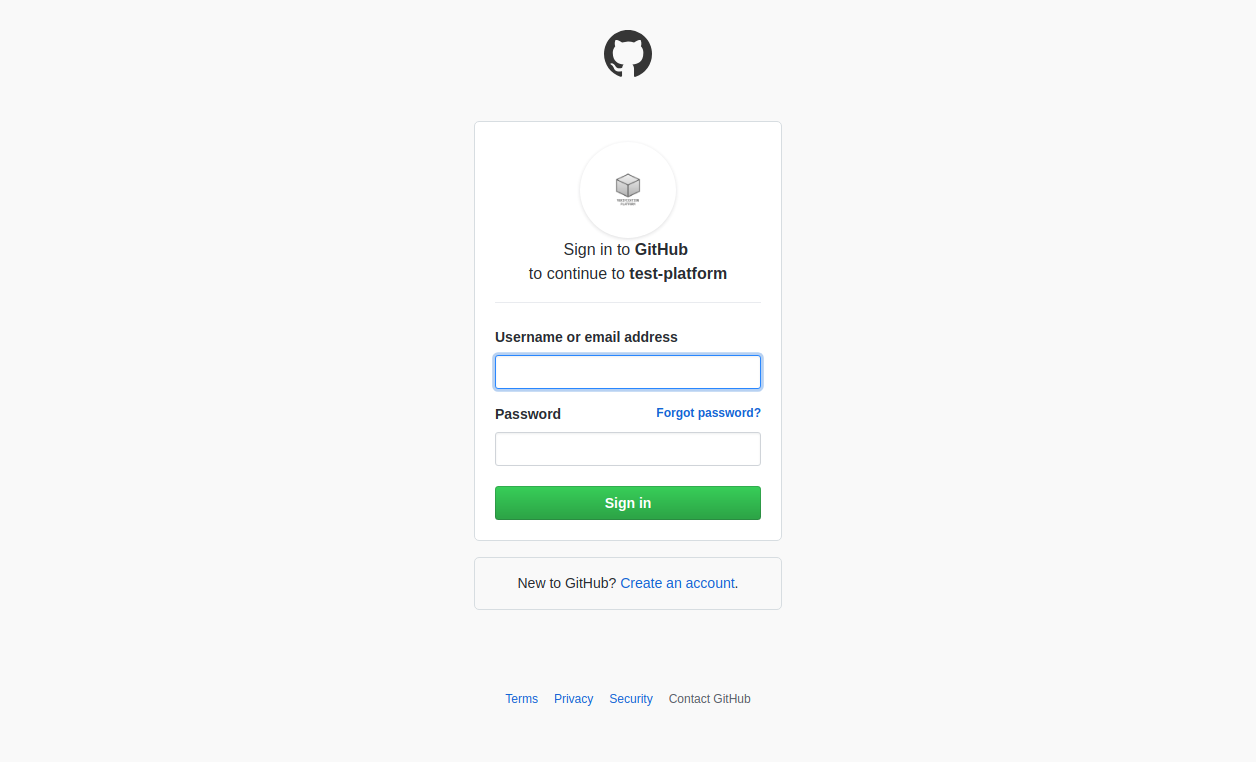
\includegraphics[width = 8cm]{chapter04/log_in_github.png}
    \caption{Ekran logowania do serwisu GitHub (źródło własne).}
    \label{fig:log_in_github}
\end{figure}

\begin{figure}[H]
    \centering
    
\includegraphics[width = 8cm]{chapter04/wait_for_login.png}
    \caption{Ekran oczekiwania na zalogowanie w ramach platformy (źródło własne).}
    \label{fig:wait_for_login}
\end{figure}

\section{Interfejs prowadzącego}

Jeśli zalogowany użytkownik posiada uprawnienia prowadzącego (administratora) po poprawnym zalogowaniu wyświetlany jest mu ekran wyboru zarządzania projektami lub podglądu postępów grup.
Ekran wyboru akcji został zamieszczony na rysunku \ref{fig:lecturer_actions}.

\begin{figure}[h]
    \centering
    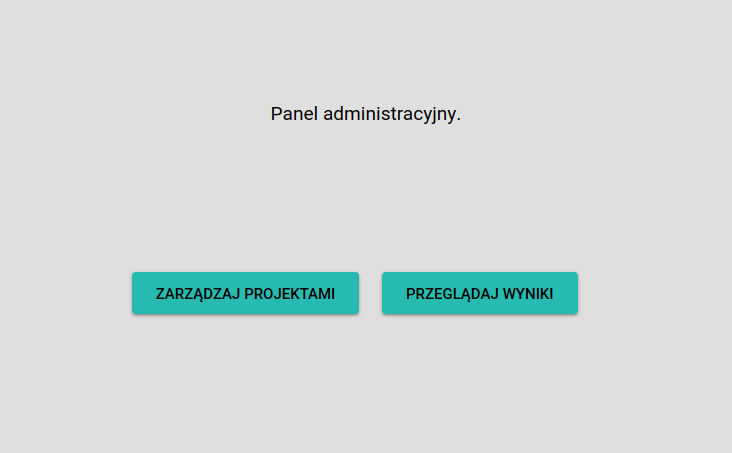
\includegraphics[width = 8cm]{chapter04/lecturer_actions.png}
    \caption{Ekran wyboru akcji dla prowadzącego (źródło własne).}
    \label{fig:lecturer_actions}
\end{figure}

Omówienie widoku zarządzania projektami znajduje się w podrozdziale \ref{lecturer-management}.
Opis interfejsu podglądu postępów studentów został zamieszczony w sekcji \ref{lecturer_preview}.

\subsection{Zarządzanie projektami}
\label{lecturer-management}

W ramach zarządzania udostępnione jest tworzenie i edytowanie projektów, w tym wyznaczanie etapów i integracji oraz dodawanie do nich przypadków testowych.
Zdefiniowanie projektu sprowadza się do:
\begin {itemize}
    \item Utworzenia nowego projektu.
    \item Dodania etapów wraz z przypadkami testowymi.
    \item Utworzenia procesów integracji wraz z przypadkami testowymi.
    \item Dodania grup projektowych.
\end {itemize}

Dla wszystkich parametrów będących plikami interfejs umożliwia dodanie ich poprzez wskazanie w oknie dialogowym ścieżki na dysku użytkownika, pod którą znajduje się plik.

Na rysunku \ref{fig:lecturer_projects_list} został przedstawiony podstawowy widok zarządzania projektami zawierający listę dostępnych projektów.
Na tym ekranie prowadzący może przejść do wybranego projektu, usunąć go lub utworzyć nowy projekt.
Lista dostępnych projektów jest posortowana alfabetycznie po ich nazwie.

\begin{figure}[h]
    \centering
    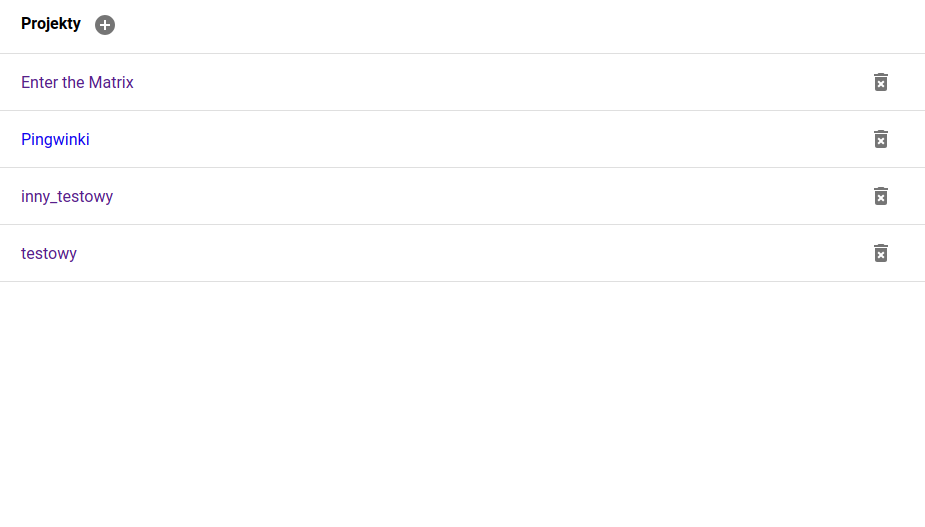
\includegraphics[width = 8cm]{chapter04/lecturer_projects_list.png}
    \caption{Interfejs prowadzącego, zarządzanie projektami - lista projektów (źródło własne).}
    \label{fig:lecturer_projects_list}
\end{figure}

Widok projektu oraz panele etapów, integracji i grup zostały omówione w ramach kolejnych sekcji.

\subsubsection{Widok projektu}

Projekt definiowany jest przez następujące dane:
\begin {itemize}
    \item Nazwę projektu, która jest jednoznaczna z nazwą katalogu na dysku, w którym przechowywane będą pliki z danymi dotyczącymi projektu.
    Nazwa jest parametrem będącym ciągiem znaków (String).
    \item Plik z opisem projektu o dowolnym formacie.
    \item Plik Dockerfile definiujący środowisko uruchomieniowe programów.
    \item Listę etapów.
    \item Listę integracji.
    \item Listę grup.
\end {itemize}

Na rysunku \ref{fig:lecturer_project_board} przedstawiono podstawowy widok projektu.

\begin{figure}[h]
    \centering
    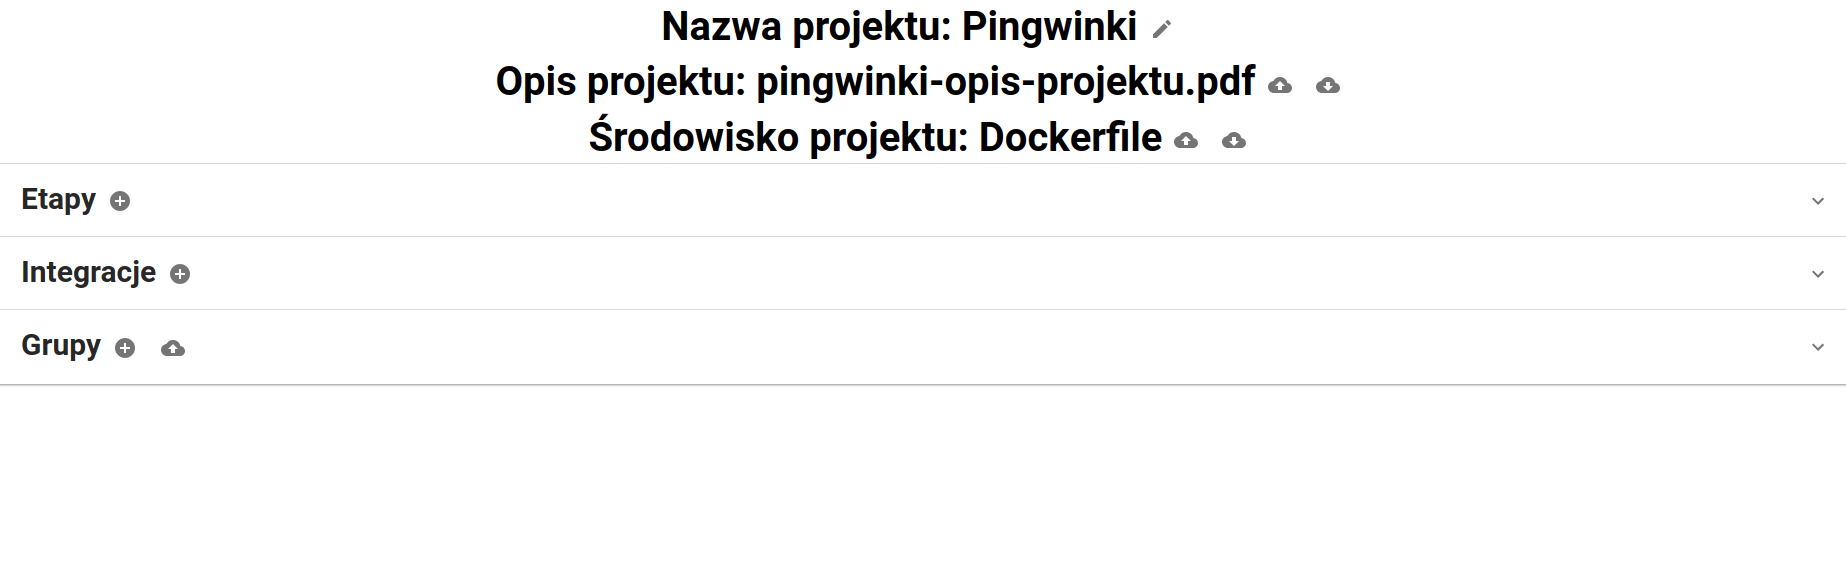
\includegraphics[width = 13cm]{chapter04/lecturer_project_board.png}
    \caption{Interfejs prowadzącego, zarządzanie projektami - widok projektu (źródło własne).}
    \label{fig:lecturer_project_board}
\end{figure}

\subsubsection{Panel etapów}

Etap definiowany jest przez następujące dane:
\begin {itemize}
    \item Nazwę etapu, która jest jednoznaczna z nazwą katalogu na dysku, w którym przechowywane będą pliki z danymi dotyczącymi etapu.
    Nazwa jest parametrem będącym ciągiem znaków (String).
    \item Plik z opisem etapu o dowolnym formacie.
    \item Metadane dotyczące etapu, takie jak:
    \begin {itemize}
        \item Data rozpoczęcia etapu.
        Data rozpoczęcia jest rozumiana jako data, od której studenci mają możliwość rozpoczęcia prac nad etapem (dostęp do opisu etapu, możliwość zaimportowania i uruchomienia swoich programów).
        \item Data zakończenia etapu.
        Data zakończenia jest rozumiana jako data, do której studenci mają możliwość zaimportowania i uruchomienia swoich programów.
        Po przekroczeniu tej daty zmian programów i ponownych uruchomień może dokonywać tylko prowadzący.
        \item Komentarz do etapu.
        Jest on dodatkową informacją widoczną tylko dla prowadzącego.
    \end{itemize}
\end {itemize}

Etapy, które nie mają zdefiniowanej daty rozpoczęcia nie są widoczne dla studentów.
Lista etapów jest posortowana rosnąco po dacie zakończenia etapu.
Interfejs umożliwia wskazanie dat poprzez ich wybór w oknie dialogowym z kalendarzem.

Na rysunku \ref{fig:lecturer_stages} został przedstawiony przykładowy panel etapów.
Komentarz do etapu wyświetlany jest po najechaniu na ikonę reprezentującą dodatkowe informacje.

\begin{figure}[h]
    \centering
    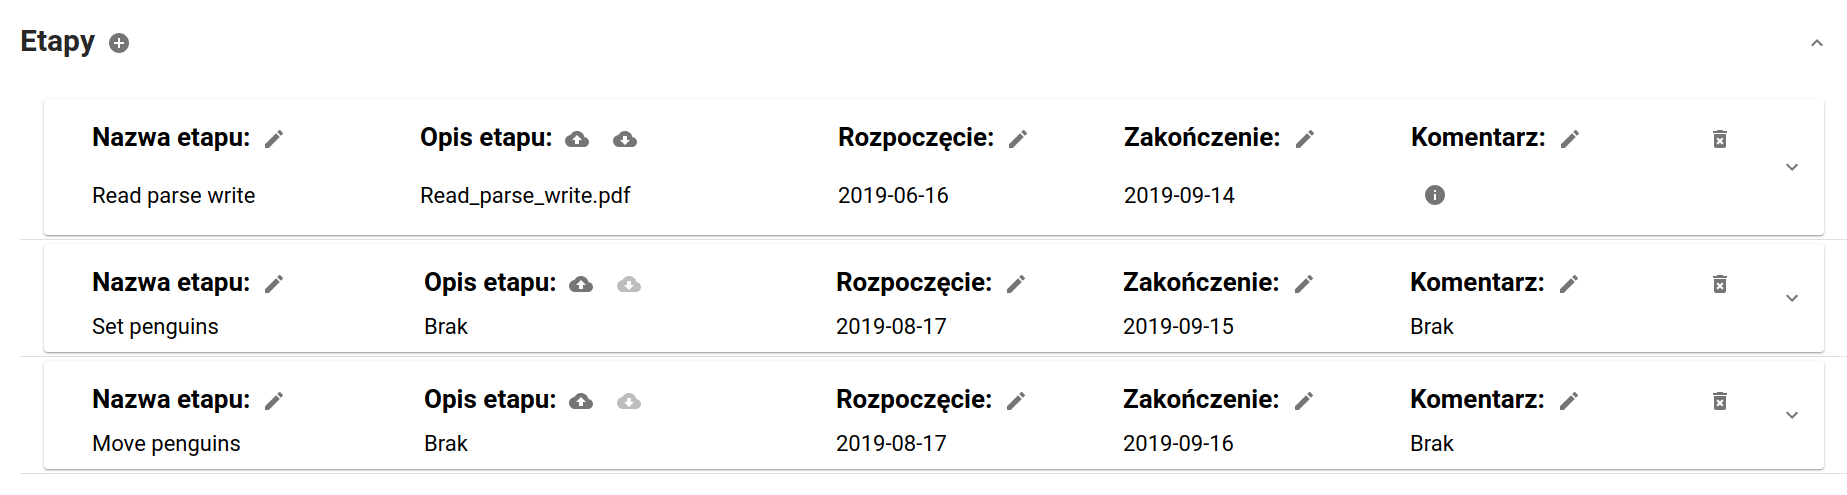
\includegraphics[width = 15cm]{chapter04/lecturer_stages.png}
    \caption{Interfejs prowadzącego, zarządzanie projektami - panel etapów (źródło własne).}
    \label{fig:lecturer_stages}
\end{figure}

W ramach panelu można dodawać, edytować oraz usuwać etapy.


Dla każdego z etapów można rozwinąć panel zawierający listę zdefiniowanych testów.
Opis uruchamianie i testowania programów studentów w ramach etapów został zamieszczony w rozdziale \ref{chapter:platform-technical}.
Pojedynczy przypadek testowy jest definiowany przez następujące dane:
\begin {itemize}
    \item Nazwę przypadku testowego, która jest jednoznaczna z nazwą katalogu na dysku, w którym przechowywane będą pliki z danymi dotyczącymi tego przypadku.
    Nazwa jest parametrem będącym ciągiem znaków (String).
    \item Parametry uruchomienia programu, podawane jako plik.
    \item Plik z danymi wejściowymi dla zadanego przypadku o dowolnym, najczęściej tekstowym, formacie.
    Plik wejściowy jest używany jako dana wejściowa dla danego przypadku testowego.
    \item Oczekiwany plik wyjściowy dla zadanego przypadku o dowolnym, najczęściej tekstowym, formacie.
    Oczekiwany plik wyjściowy jest używany do porównania wyniku otrzymanego w rezultacie działania programów studentów i na jego podstawie oceniana jest poprawność programów.
\end {itemize}

Rysunek \ref{fig:lecturer_stages_tests} przedstawia przykładowy panel zawierający definicje testów dla etapu.

\begin{figure}[h]
    \centering
    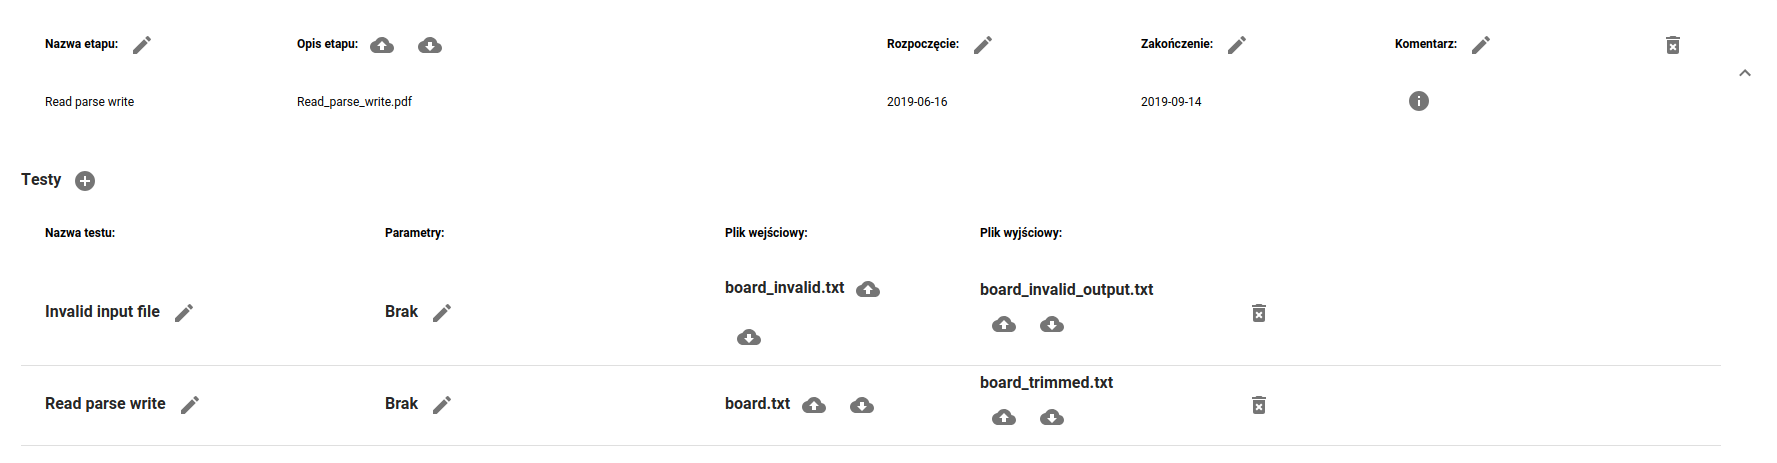
\includegraphics[width = 15cm]{chapter04/lecturer_stages_tests.png}
    \caption{Interfejs prowadzącego, zarządzanie projektami - panel testów dla etapu (źródło własne).}
    \label{fig:lecturer_stages_tests}
\end{figure}

W ramach każdego z paneli można dodawać, edytować oraz usuwać przypadki testowe.

\subsubsection{Panel integracji}

Proces integracji jest definiowany przez następujące dane:
\begin {itemize}
    \item Nazwę procesu, która jest jednoznaczna z nazwą katalogu na dysku, w którym przechowywane będą pliki z danymi dotyczącymi tego procesu.
    Nazwa jest parametrem będącym ciągiem znaków (String).
    \item Priorytetyzowaną listę etapów, które zostaną wykonane kolejno w ramach procesu integracji.
    \item Komentarz do procesu integracji.
    Jest on dodatkową informacją widoczną tylko dla prowadzącego.
\end {itemize}

Na rysunku \ref{fig:lecturer_integrations} został przedstawiony przykładowy panel integracji.

\begin{figure}[h]
    \centering
    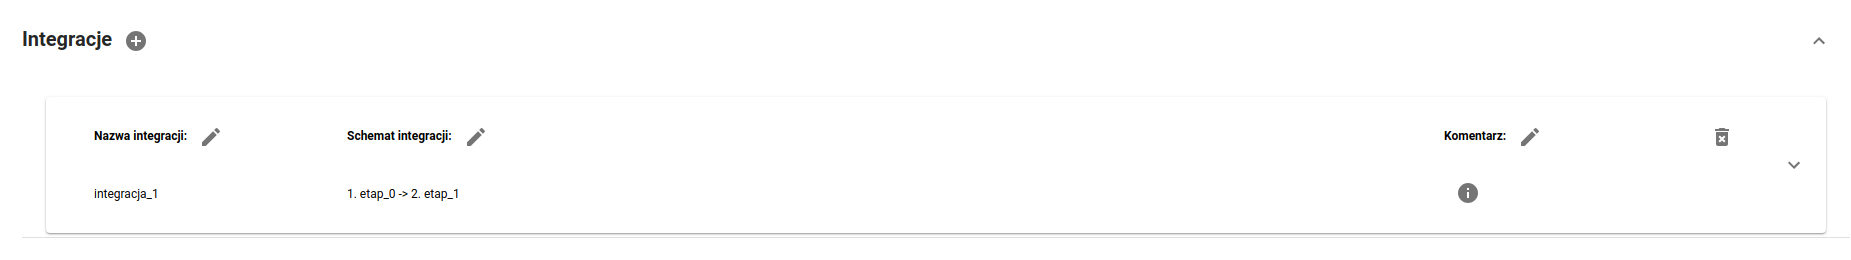
\includegraphics[width = 15cm]{chapter04/lecturer_integrations.png}
    \caption{Interfejs prowadzącego, zarządzanie projektami - panel integracji (źródło własne).}
    \label{fig:lecturer_integrations}
\end{figure}

Dla każdej z integracji można rozwinąć panel zawierający listę zdefiniowanych testów.
Opis uruchamianie i testowania programów studentów w ramach procesu integracji został zamieszczony w rozdziale \ref{chapter:platform-technical}.
Pojedynczy przypadek testowy jest definiowany przez następujące dane:
\begin {itemize}
    \item Nazwę przypadku testowego, która jest jednoznaczna z nazwą katalogu na dysku, w którym przechowywane będą pliki z danymi dotyczącymi tego przypadku.
    Nazwa jest parametrem będącym ciągiem znaków (String).
    \item Parametry uruchomienia programu, podawane jako pliki.
    Dla każdego z etapów integracji podawane są oddzielne parametry wykonania w ramach jednego testu.
    \item Plik z danymi wejściowymi dla zadanego przypadku o dowolnym, najczęściej tekstowym, formacie.
    Plik wejściowy jest używany jako dana wejściowa dla danego przypadku testowego i jest pojedynczy w ramach jednego testu.
    \item Oczekiwany plik wyjściowy dla zadanego przypadku o dowolnym, najczęściej tekstowym, formacie.
    Oczekiwany plik wyjściowy jest używany do porównania wyniku otrzymanego w rezultacie działania programów studentów i na jego podstawie oceniana jest poprawność programów.
    Oczekiwany plik wyjściowy jest pojedynczy w~ramach jednego testu.
\end {itemize}

\begin{figure}[h]
    \centering
    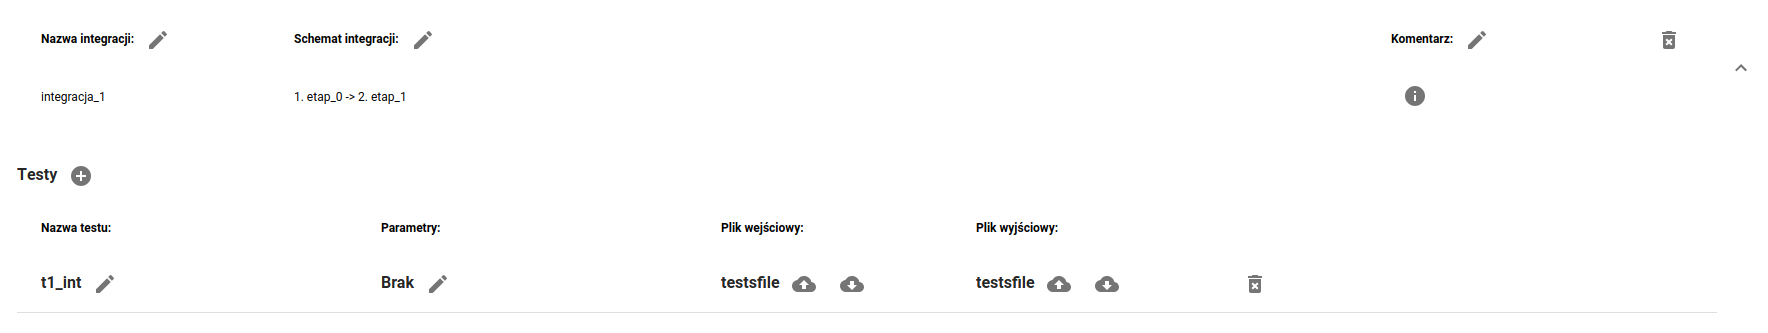
\includegraphics[width = 15cm]{chapter04/lecturer_integrations_tests.png}
    \caption{Interfejs prowadzącego, zarządzanie projektami - panel testów dla integracji (źródło własne).}
    \label{fig:lecturer_integrations_tests}
\end{figure}

W ramach każdego z paneli można dodawać, edytować oraz usuwać przypadki testowe.

\subsubsection{Panel grup}

W ramach panelu prowadzący ma możliwość utworzenia grup projektowych oraz przypisania do nich studentów.
Na rysunku \ref{fig:lecturer_groups} zamieszczono widok rozwiniętego panelu grup.
Kolejny rysunek \ref{fig:lecturer_students_in_group} przedstawia rozwiniętą listę studentów przypisanych do danego zespołu.

\begin{figure}[h]
    \centering
    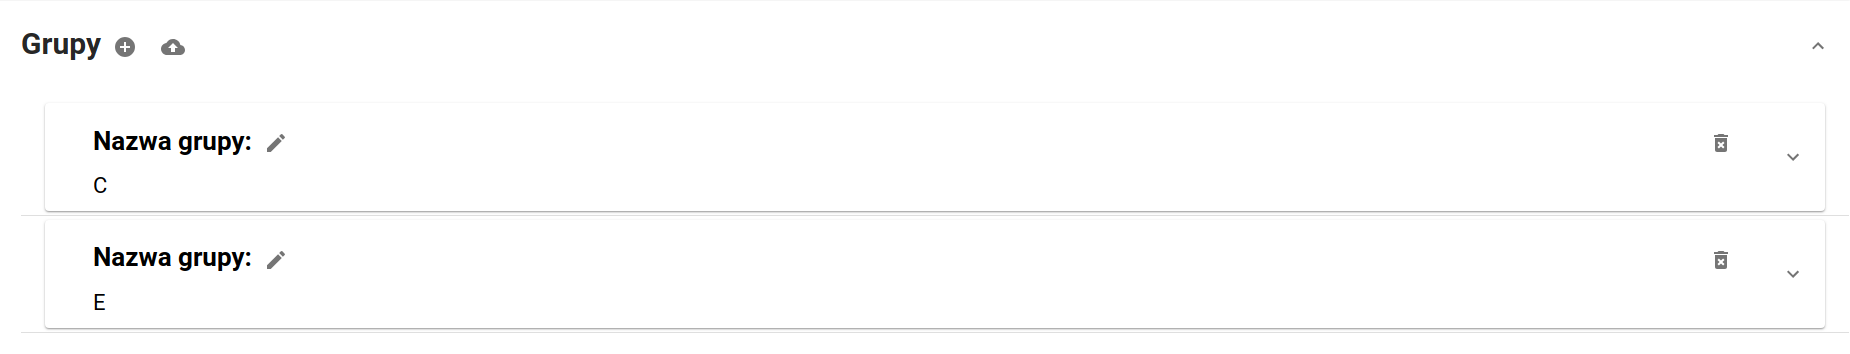
\includegraphics[width = 13cm]{chapter04/lecturer_groups.png}
    \caption{Interfejs prowadzącego, zarządzanie projektami - panel grup (źródło własne).}
    \label{fig:lecturer_groups}
\end{figure}

\begin{figure}[h]
    \centering
    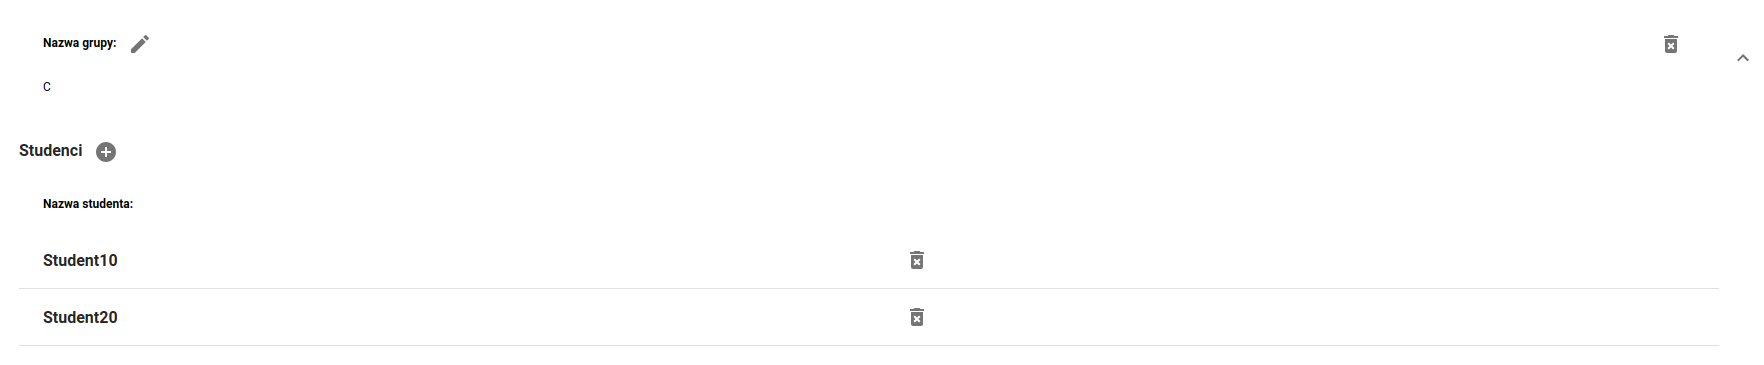
\includegraphics[width = 13cm]{chapter04/lecturer_students_in_group.png}
    \caption{Interfejs prowadzącego, zarządzanie projektami - panel grupy wraz z przypisanymi studentami (źródło własne).}
    \label{fig:lecturer_students_in_group}
\end{figure}

Utworzenie grup projektowych może zostać zrealizowane na dwa sposoby.
Pierwszy z nich to manualne utworzenie grup definiowanych przez nazwę i dodanie kolejnych studentów w oknie dialogowym.
Aby dodać grupy manualnie należy użyć przycisku ”+” znajdującego się obok etykiety \textit{Grupy}.
Drugim sposobem definicji grup jest wczytanie ich bezpośrednio z pliku w formacie JSON.
Przykład struktury akceptowalnego pliku został zamieszczony w podrozdziale \ref{adding_project_groups}.
W celu wczytania grup z pliku należy użyć przycisku wgrywania danych znajdującego się obok etykiety \textit{Grupy}.

W ramach panelu umożliwiona jest edycja grup i przypisanych do nich studentów.

\subsection{Podgląd postępów studentów}
\label{lecturer_preview}

Panel podglądu postępów studentów umożliwia:
\begin {itemize}
    \item Sprawdzenie statusu prac w ramach etapów i integracji dla każdej ze zdefiniowanych grup projektowych.
    \item Uruchomienie programów.
    \item Edycję danych (programu, raportu, kodu) przez prowadzącego.
    \item Pobranie pliku zawierającego statystyki uruchomień dla integracji i etapów.
\end {itemize}

Prowadzący ma możliwość edycji danych studentów z uprawnieniami administratora.
Pozwalają one między innymi na zmianę wprowadzonych przez studentów informacji i~plików po upływie terminów realizacji poszczególnych etapów.
Są to uprawnienia, które nie powinny być nadużywane przez prowadzącego, jednak mogą okazać się użyteczne w~wyjątkowych sytuacjach.

Na rysunku \ref{fig:lecturer_preview_projects_list} został przedstawiony podstawowy widok zarządzania projektami zawierający listę dostępnych projektów.
Poprzez ten ekran prowadzący może przejść do wybranego projektu.
Lista dostępnych projektów jest posortowana alfabetycznie po ich nazwie.

\begin{figure}[h]
    \centering
    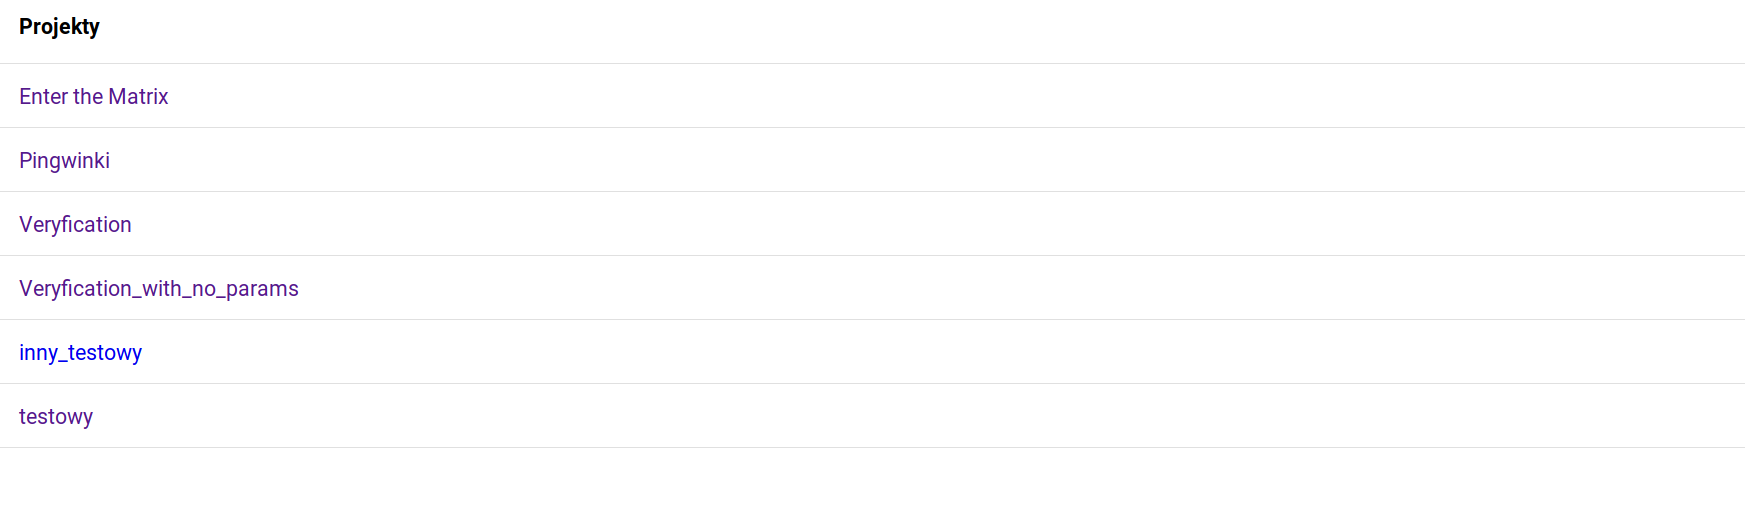
\includegraphics[width = 13cm]{chapter04/lecturer_preview_projects_list.png}
    \caption{Interfejs prowadzącego, podgląd postępów - lista projektów (źródło własne).}
    \label{fig:lecturer_preview_projects_list}
\end{figure}

Po przejściu do odpowiedniego projektu wyświetlany jest ekran z listą grup i przypisanych do nich studentów.
Poprzez ten ekran prowadzący może przejść do rezultatów wybranego zespołu.
Lista grup jest posortowana alfabetycznie po nazwie.
Przykładowy ekran wyboru zespołu projektowego został zamieszczony na rysunku \ref{fig:lecturer_preview_groups}.

\begin{figure}[h]
    \centering
    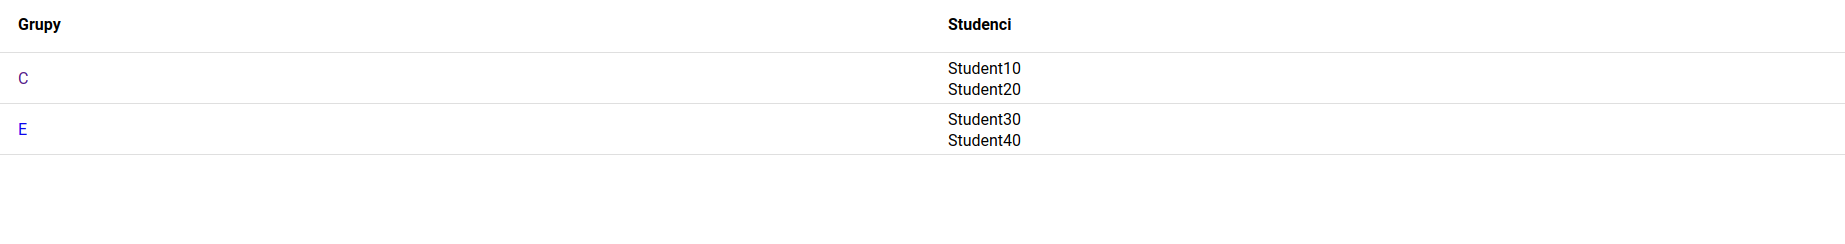
\includegraphics[width = 13cm]{chapter04/lecturer_preview_groups.png}
    \caption{Interfejs prowadzącego, podgląd postępów - lista grup (źródło własne).}
    \label{fig:lecturer_preview_groups}
\end{figure}

Na rysunku \ref{fig:lecturer-interface-preview} został przedstawiony widok podglądu postępów dla grupy studentów.
W ramach widoku można:
\begin{itemize}
    \item Pobrać opis projektu.
    \item Pobrać środowisko uruchomieniowe.
    \item Uruchomić programy oraz podejrzeć wyniki dla kolejnych etapów.
    \item Uruchomić procesy integracji oraz przejrzeć rezultaty ich wykonania.
\end{itemize}

\begin{figure}[h]
    \centering
    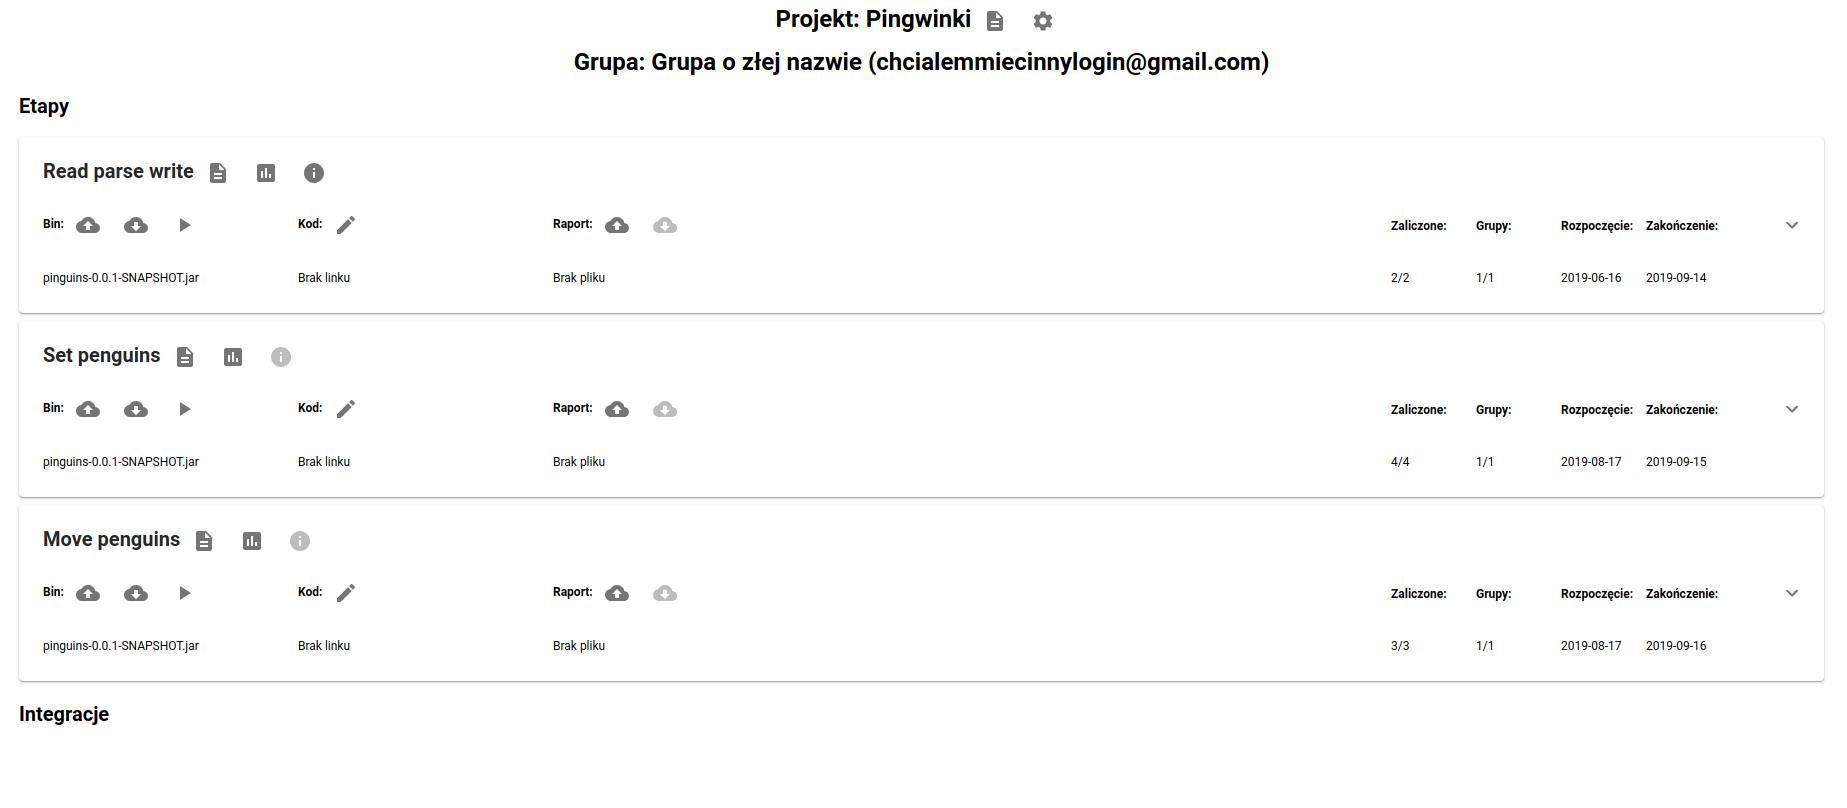
\includegraphics[width = 13cm]{chapter04/lecturer_interface_preview.png}
    \caption{Interfejs prowadzącego, podgląd postępów studentów - podgląd projektu dla grupy (źródło własne).}
    \label{fig:lecturer-interface-preview}
\end{figure}


\subsubsection{Pogląd postępów w ramach etapów}

Panel podglądu postępów w ramach etapu zawiera informacje o statusie prac w ramach każdego ze zdefiniowanych etapów.
Widok został przedstawiony na rysunku \ref{fig:lecturer-preview-stage}.
Umożliwia on prowadzącemu:
\begin {itemize}
    \item Pobranie opisu etapu.
    \item Pobranie statystyk z uruchomienia programów.
    \item Podejrzenie komentarza.
    \item Uruchomienie, pobranie i wgranie programu.
    \item Edycję linku do kodu.
    \item Pobranie i wgranie raportu.
\end {itemize}

Panel zawiera również dodatkowe informacje takie jak:
\begin{itemize}
    \item Status zaliczenia etapu określający ile ze wszystkich testów zostało zaliczone przez grupę (pole \textit{Zaliczone}).
    \item Status zaliczenia etapu w ramach wszystkich grup mówiący ile zespołów zaliczyło dane zadanie (pole \textit{Grupy}).
    \item Data rozpoczęcia etapu.
    \item Data zakończenia etapu.
\end{itemize}

\begin{figure}[h]
    \centering
    
\includegraphics[width = 13cm]{chapter04/lecturer_preview_stage.png}
    \caption{Interfejs prowadzącego, podgląd postępów studentów - podgląd etapu (źródło własne).}
    \label{fig:lecturer-preview-stage}
\end{figure}

Po rozwinięciu widoku etapu widoczny jest dodatkowo panel wyników testów (patrz rysunek \ref{fig:lecturer-preview-stage-tests}).
Zawiera on informacje o uruchomionych przypadkach testowych w tym:
\begin{itemize}
    \item Nazwę przypadku testowego.
    \item Status uruchomienia. W przypadku poprawnego rezultatu testu wyświetlany jest \textit{SUCCESS}, dla niewłaściwego wyniku widoczny jest \textit{FAILURE}.
    \item Komunikat błędu.
\end{itemize}

Panel pozwala na pobranie:
\begin{itemize}
    \item Logów z wykonania programu dla zadanego przypadku testowego.
    \item Parametrów wywołania.
    \item Pliku wejściowego.
    \item Oczekiwanego pliku wyjściowego dla testu.
\end{itemize}

\begin{figure}[h]
    \centering
    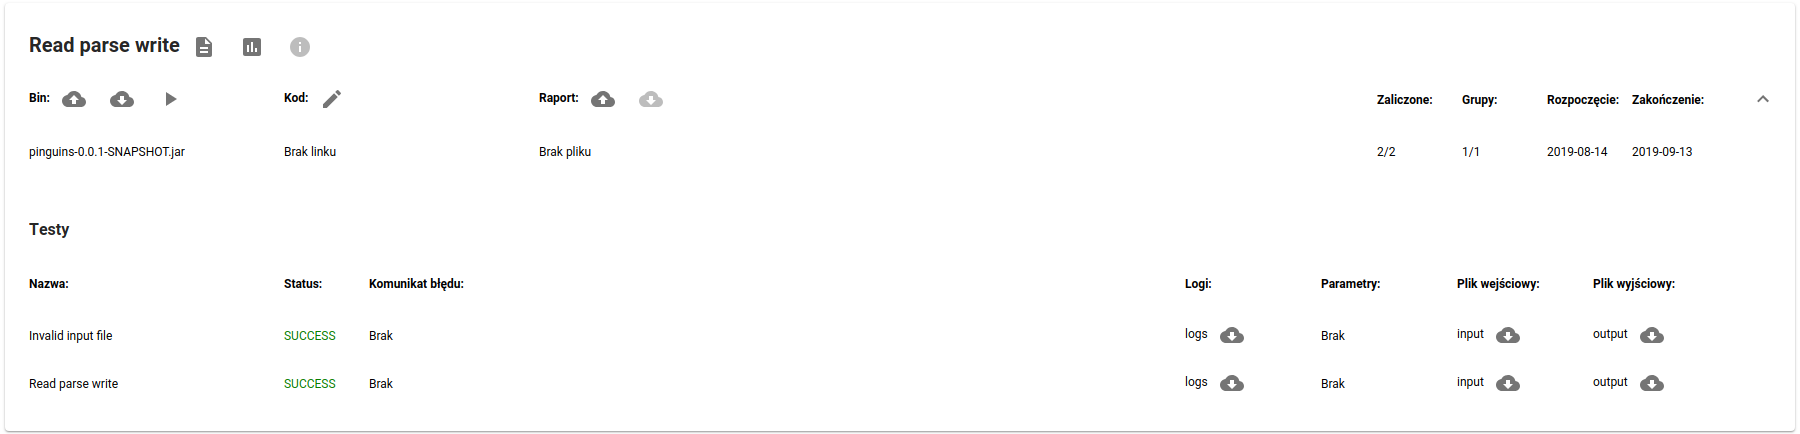
\includegraphics[width = 13cm]{chapter04/lecturer_preview_stage_tests.png}
    \caption{Interfejs prowadzącego, podgląd postępów studentów - podgląd wyników testów dla etapu (źródło własne).}
    \label{fig:lecturer-preview-stage-tests}
\end{figure}

\subsubsection{Pogląd postępów w ramach integracji}

Panel podglądu postępów w ramach integracji zawiera informacje o statusie prac dla każdego ze zdefiniowanych procesów integracji.
Przykładowy widok został zamieszczony na rysunku \ref{fig:lecturer-preview-integration}.
Panel podglądu postępów w ramach integracji umożliwia prowadzącemu:
\begin {itemize}
    \item Pobranie statystyk z uruchomienia integracji.
    \item Podejrzenie komentarza.
    \item Uruchomienie integracji.
\end {itemize}

Panel zawiera również dodatkowe informacje takie jak:
\begin{itemize}
    \item Schemat integracji obrazujący, które z etapów i w jakiej kolejności zostaną uruchomione w~ramach procesu integracji.
    \item Status zaliczenia integracji określający ile ze wszystkich testów zostało zaliczone przez grupę (pole \textit{Zaliczone}).
    \item Status zaliczenia integracji w ramach wszystkich grup mówiący ile zespołów zaliczyło dane zadanie (pole \textit{Grupy}).
\end{itemize}

\begin{figure}[h]
    \centering
    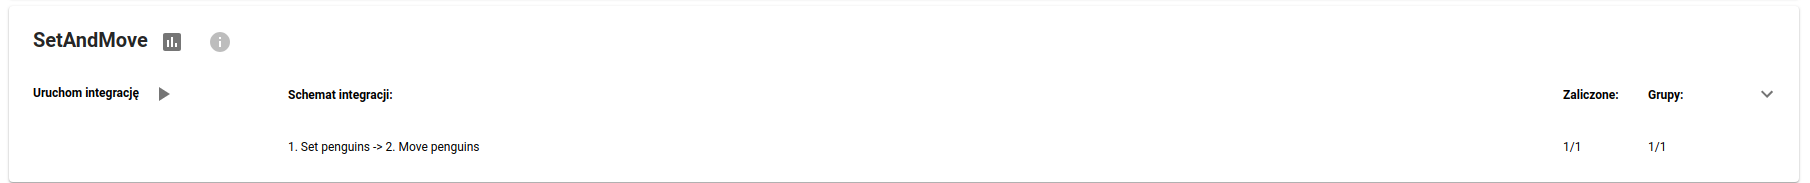
\includegraphics[width = 13cm]{chapter04/lecturer_preview_integration.png}
    \caption{Interfejs prowadzącego, podgląd postępów studentów - podgląd integracji (źródło własne).}
    \label{fig:lecturer-preview-integration}
\end{figure}

Po rozwinięciu widoku integracji widoczny jest dodatkowo panel wyników testów (patrz rysunek \ref{fig:lecturer-preview-integration-tests}).
Zawiera on informacje o uruchomionych przypadkach testowych w~tym:
\begin{itemize}
    \item Nazwę przypadku testowego.
    \item Status uruchomienia. W przypadku poprawnego rezultatu testu wyświetlany jest \textit{SUCCESS}, dla niewłaściwego wyniku widoczny jest \textit{FAILURE}.
    \item Komunikat błędu.
\end{itemize}

\begin{figure}[h]
    \centering
    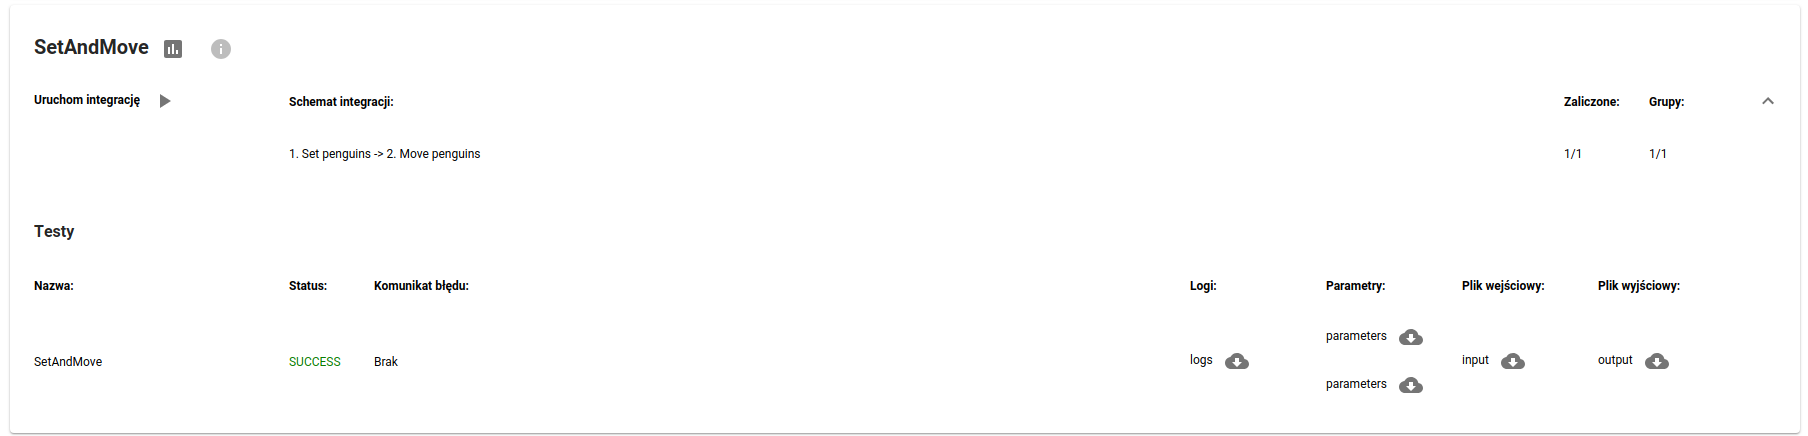
\includegraphics[width = 13cm]{chapter04/lecturer_preview_integration_tests.png}
    \caption{Interfejs prowadzącego, podgląd postępów studentów - podgląd wyników testów dla integracji (źródło własne).}
    \label{fig:lecturer-preview-integration-tests}
\end{figure}

Panel pozwala na pobranie:
\begin{itemize}
    \item Logów z wykonania programu dla zadanego przypadku testowego.
    \item Parametrów wywołania dla każdego z etapów wchodzących w skład integracji.
    \item Pliku wejściowego.
    \item Oczekiwanego pliku wyjściowego dla testu.
\end{itemize}





\section{Interfejs studenta}
TODO: Dodać rysunki

Po zalogowaniu do platformy z uprawnieniami studenta użytkownikowi wyświetlany jest ekran dostępnych dla niego projektów.
Są one posortowane alfabetycznie po nazwie.
Na rysunku \ref{fig:student_projects} został przedstawiony podstawowy widok dla interfejsu studenta.

TODO: dodać rysunek

Po przejściu do wybranego projektu wyświetalny jest panel postępów dla grupy projektowej, do której jest przypisany student.
Przykładowy ekran został przedstawiony na rysunku \ref{fig:student_project}.

TODO: dodać rysunek

Warto zauważyć, że interfejs jest bardzo podobny do widoku podglądu wyników w ramach grupy projektowej dla prowadzącego.
Student ma jednak pewne ograniczenia co do akcji wykonywanych w ramach interfejsu.
Nie może on między innymi podejrzeć komentarzy i pobrać statystyk uruchomienia programów dla zadań.
Student nie ma również możliwości zmiany zaimportowanych danych po upływie terminu zakończenia etapu.

\subsubsection{Pogląd postępów w ramach etapów}

Na rysunku \ref{fig:student_stage_view} został przedstawiony podgląd postępów w ramach etapów dla studenta.
W ramach tego panelu udostępnione są wszystkie akcje związane z załączeniem i edycją danych dotyczących każdego z zadań.
Student ma także umożliwiony pełny podgląd rezultatów uruchomienia aplikacji dla kolejnych przypadków testowych.

TODO: dodać rysunek

\subsubsection{Pogląd postępów w ramach integracji}

Student po zakończeniu odpowiedniej liczby etapów wchodzących w skład zdefiniowanego procesu integracji ma możliwość uruchomienia go.
Rezultat działania procesu jest reprezentowany podobnie jak na widoku podglądu wyników dla prowadzącego.
Przykładowy panel został przedstawiony na rysunku \ref{fig:student_integration_view}.
Różni się on od widoku prowadzącego brakiem przycisku do pobrania statystyk i wyświetlenia komentarza.

TODO: dodać rysunek